\documentclass[a6paper, 10pt, twoside]{article}
%\usepackage[T1]{fontenc}
\usepackage[british]{babel}
\usepackage[utf8]{inputenc}
\usepackage{float, graphicx,amsmath,amsfonts,cite,enumerate,tabularx}
\usepackage[final]{pdfpages}
\usepackage{wrapfig}
\usepackage[margin=0.3in]{geometry}
\usepackage{sidspaltHack}
\usepackage{digital}

\setlength{\oddsidemargin}{-0.37in}
\setlength{\evensidemargin}{-0.47in}
\setlength{\textwidth}{215pt}

\pagestyle{empty}

\begin{document}
\nysida{7}{1}
\noindent
\chaptertitlenobr{H$\eta$}{Visor till andra drycker}
\small
\begin{center}
\songtitle{$\eta1$}{Skål för vattnet} 
\mel{Rule Britannia}
\end{center}
\begin{lyrics}
I Spanien hör det till god ton och etikett\\
att gå omkring och skryta vitt och brett.\\
De trodde att de skulle slå oss lätt!
\vspace{5pt}\\
Men vi är modesta.\\
Ja, vår profil är låg,\\
men vi är de som väger tyngst på havets våg!
\vspace{5pt}\\
Skål för vattnet, tjoho för H$_2$O!\\
Skål för ön där bara blyga britter bo!\\
Skål för vattnet som gör vår flotta stark,\\
hell allt vatten som ger flyt åt vår monark!
\end{lyrics}
\auth{Vattenfysikalen Shakespeare 1990}

\nysida{7}{2}
\noindent
\begin{center}
\songtitle{$\eta2$}{En kan dricka vatten}
\mel{Vi äro musikanter}
\end{center}
\begin{lyrics}
En kan dricka vatten, \\
mjölk, och gammalt flott.\\
Men vi dricker hellre\\
sådant som är gott.
\vspace{5pt}\\
Vi kan dricka brännvin, öl och billigt vin.\\
Vi kan dricka olja och bensin.
\vspace{5pt}\\
Och vi kan svepa islandshästar,\\
mockavästar när vi festar.\\
Vi kan svepa svavelsyra på vår yra fest.
\vspace{5pt}\\
Vi kan häva kvicksilver och helium.\\
Vi kan häva ost och vardagsrum.
\vspace{5pt}\\
Och vi kan supa bomfadderalla,\\
bomfadderalla, skål på Er alla!\\
Vi kan supa andra hållet, andra hållet med. 
\end{lyrics}
\auth{n$\emptyset$llespexet 1995}

\nysida{7}{3}
\noindent
\begin{center}
\songtitle{$\eta3$}{Nu tar vi rom}
\mel{Deck the hall}
\end{center}
\begin{lyrics}
Här på skeppet rinner rommen,\\
lalalalala lalalala!\\
Rom till varje nyankommen,\\
lalalalala lalalala!\\
Höj nu bägarn eller spannen,\\
lalala lalala lalala!\\
Sjung och skåla sen med grannen,\\
lalalalala lalalala!
\vspace{5pt}\\
Om än rommen smakar som en,\\
lalalalala lalalatrin\\
är till vommen rommen kommen\\
jajajajamaicas brända vin!\\
ROM och RAM och rom och cola,\\
lalalalax lägger också rom.\\
"Rom och mjölke" vill vi vråla.\\
Allalala vägar bär till rom! 
\end{lyrics}
\auth{Fysikalen Shakespeare 1990}
\begin{center}
\songtitle{$\eta4$}{Däj-o}
\mel{Banana boat song}
\end{center}
\begin{lyrics}
$\|$: Däj-o, däääj-o\\
Daylight come, and me wan' go home. :$\|$\\
Work all night on a drink of rum.\\
Daylight come, and me wan' go home\\
Stack the banana till the morning come.\\
Daylight come, and me wan' go home
\vspace{5pt}\\
$\|$: Dääj-o, däääj-o\\
Daylight come, and me wan' go home :$\|$\\
Däääj-o! 
\end{lyrics}

\nysida{7}{5}
\noindent
\begin{center}
\songtitle{$\eta5$}{Mjölk}
\mel{Trink, trink}
\end{center}
\begin{lyrics}
Mjölk, mjölk vi vill ha mjölk,\\
det är en underbar dryck.\\
Mjölk, mjölk vi vill ha mjölk,\\
det är vår senaste nyck.\\
Hämta din spann, mjölka din get,\\
ge mig en klunk utav det.\\
Slut upp i kampen för helnykterhet.\\
Mjölk är det bästa jag vet!
\end{lyrics}
\begin{figure}[!h]
\hfill
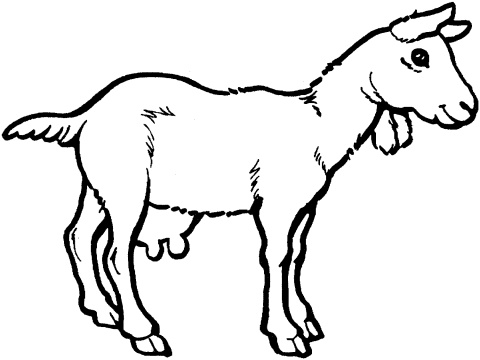
\includegraphics[width=0.5\textwidth]{goat.png}
\end{figure}
\begin{center}
\songtitle{$\eta6$}{Mjölksång}
\mel{Mors lilla Olle}
\end{center}
\begin{lyrics}
Vad dom kan göra i vårt mejeri!\\
Mjölk kan dom tillverka med grejer i.\\
Lättmjölk och folkmjölk och starkmjölk är bra.\\
Dom ska vi dricka imorgon, hurra!
\end{lyrics}

\nysida{7}{7}
\noindent
\begin{center}
\songtitle{$\eta7$}{Hyllningsvisa till absinten}
\mel{Come All Ye Faithful}
\end{center}
\begin{lyrics}
Var är absinten,\\
illgrön liksom minten,\\
som skänker galenskap åt var teknolog?
\vspace{5pt}\\
(Vi) är för banala, nästan helt normala.\\
Ja, vi vill bli unika, ja rent av magnifika,\\
helt enkelt gudalika och värda en skål!
\vspace{5pt}\\
Här är absinten,\\
illgrön liksom minten\\
som ger oss stirrig blick och rufsigt hår,
\vspace{5pt}\\
dessutom kindfärg liksom August Strindberg.\\
För att bli kreativa har vi bli'tt addiktiva,\\
snart blir vi högaktiva; vi tar oss en tår! 
\end{lyrics}
\auth{Sing-Sing Singers 2000}

\nysida{7}{8}
\noindent
\begin{center}
\songtitle{$\eta8$}{Schottis på Valhall}
\end{center}
\begin{lyrics}
Opp och hoppa, Tor.\\
Slå på trumman, bror.\\
Det är dans här på Valhall i natt.\\
Uti Fröjas sal\\
står vår asabal.\\
Opp och hoppa fast Oden har spatt.\\
Slå i mera mjöd.\\
Det får bli min död.\\
Nej, se där är ju Idun min skatt.\\
Min Valkyria kom hit\\
till vår midvinterrit.\\
Opp och hoppa på Valhall i natt.
\vspace{5pt}\\
Höder han hade hiskelig hicka.\\
Balder den bota med ingefärsdricka.\\
Vred vart väl Ving-Tor, vakna och vråla.\\
Brage bråka och Skade hon skrek:
\vspace{5pt}\\
Opp och hoppa, Tor... 
\end{lyrics}
\auth{Ulf Peder Olrog}

\nysida{7}{9}
\noindent
\begin{center}
\songtitle{$\eta9$}{Häflåten}
\mel{Midnatt råder}
\end{center}
\begin{lyrics}
Yoghurt, yoghurt,\\
fyller oss till brädden,\\
oss till brädden.\\
Gurglar härligt samman där med grädden,\\
där med grädden.\\
Gräddfil kräver att vi törstigt häfver:\\
Mjölk! Mjölk! Mjölk!
\end{lyrics}
\vspace{40pt}
\begin{center}
\songtitle{$\eta10$}{Kaffe}
\mel{Du ska få min gamla cykel när jag dör}
\end{center}
\begin{lyrics}
Kaffe, kaffe, kaffe,\\
konjak och likör,\\
ger åt alla här ett mycket gott humör.\\
På det ska ni ge er katten,\\
vi skall sitta hela natten,\\
dricka kaffe, kaffe, konjak och likör.
\end{lyrics}

\nysida{7}{11}
\noindent
\begin{center}
\songtitle{$\eta11$}{Whiskyn}
\mel{Längtan till landet}
\end{center}
\begin{lyrics} 
Whiskyn är förädling utav ölet,\\
destilleras, lagras flera år.\\
En mästardryck, full av gamla anor\\
den är glasklart barens bästa tår.
\vspace{5pt}\\
Drycken njutas bäst uti kristallglas\\
aldrig mer än fyror på en gång.\\
En kultiverad dryck som saknar like.\\
Vi hyllar alla whiskys med en sång.
\end{lyrics}
\auth{Jan Engshagen, 2011}
\begin{center}
\songtitle{$\eta12$}{1, 2, 3, Whisky!}
\mel{Siffersången (Fem myror)}
\end{center}
\begin{lyrics} 
Glenlivet,\\
Highland Park,\\
Glegoyne,\\
Glenmorangie,\\
Oban,\\
Isle of Jura,\\
Lagavulin, Bowmore, Ardbeg\\
** Laphroig!\\
Talisker,\\
Macallan,\\
Knockando,\\
Glenfarclas,\\
Clynelish!
\end{lyrics}
\auth{Didrik Lundberg, 2011}

\nysida{7}{13}
\noindent
\begin{center}
\songtitle{$\eta13$}{Kahlua}
\mel{Kalinka}
\end{center}
\begin{lyrics}
Vi söker våra rötter,\\
dricker allt som rött är.\\
Upphäver sedan glatt vårt röda tjut.
\vspace{5pt}\\
Vi söker våra rötter,\\
dricker allt som rött är.\\
Vill vi ha vodka till? Ja, Absolut!
\vspace{5pt}\\
$\|$: Kahlua, kahlua, kahlua ska i\\
med vodka och grädde rör med frenesi.\\
White Russian, White Russian, \\
White Russian det bli.\\
Den dryck som har blivit vårt livselixir. :$\|$
\end{lyrics}
\auth{Fysikalen Anastasia 2004}

\end{document}